\part{Hints and solutions to exercises}



\subsection*{Sheet 1.}

\begin{exercise} \textbf{\textit{Abelian structure of the cobordism group}}\\
Show that the disjoint union induces an abelian group structure on the cobordism group \(\Omega_n\).
\end{exercise}

\noindent First we note that, under the disjoint union, each element of $\Omega_n$ is its own inverse, i.e. $a\sqcup a=\emptyset$. Using multiplicative notation (since we prefer not to use the standard additive notation before we know we are dealing with an abelian group) we have $ab=ab(ba)(ba)=a(bb)aba=(aa)ba=ba$ using associativity, hence proving that the group structure is abelian.

\hspace{1cm}

\begin{exercise} \textbf{\textit{Orientable Manifolds}}
\begin{enumerate}[label=(\alph*)]
    \item Show that the circle $S^1$ is an orientable manifold. 
    \item Show that the sphere $S^2$ is an orientable manifold. 
    \item Show that the total space of the tangent bundle of a smooth n-manifold is an orientable
manifold. 
\end{enumerate}
\end{exercise}

\noindent A way of proving a manifold is orientable is finding a local trivialisation of the tangent bundle. To do this we first pick an open cover and then prove that the transition functions are orientation preserving (we understand what orientation means in Euclidean space). 

\begin{enumerate}[label=(\alph*)]
    \item For $S^1$ we can use an open cover inspired by the universal cover. We choose $U_1=(-\pi,\pi)$ and $U_2=(0,2\pi)$ along with the maps $\varphi_1:x\mapsto e^{ix}$ and $\varphi_2:x\mapsto e^{ix}$, respectively. Looking at the transition map $\varphi_1^-1\circ \varphi_2$ we get a map between $(0,\pi)\cup (\pi,2\pi)\to (0,\pi)\cup (-\pi,0)$ acting like the identity on the first constituent interval and like the identity plus $2\pi$ on the second one. By symmetry, we have a similar situation for the other transition function. Therefore, the differential acts by the identity on the tangent spaces, and so this has determinant $1>0$. Thus we conclude that $S^1$ is orientable, as required.
    \item \textbf{Attempt 1:} We try doing this using the standard stereographic projections from the north and south poles, respectively, as an atlas. Then, it is well known that the (both!) transition maps are simply circle inversions on $\R^2\setminus \{0\}$. See the picture below for clarification (this is a simple exercise in standard Euclidean geometry).
    
    \begin{center}
            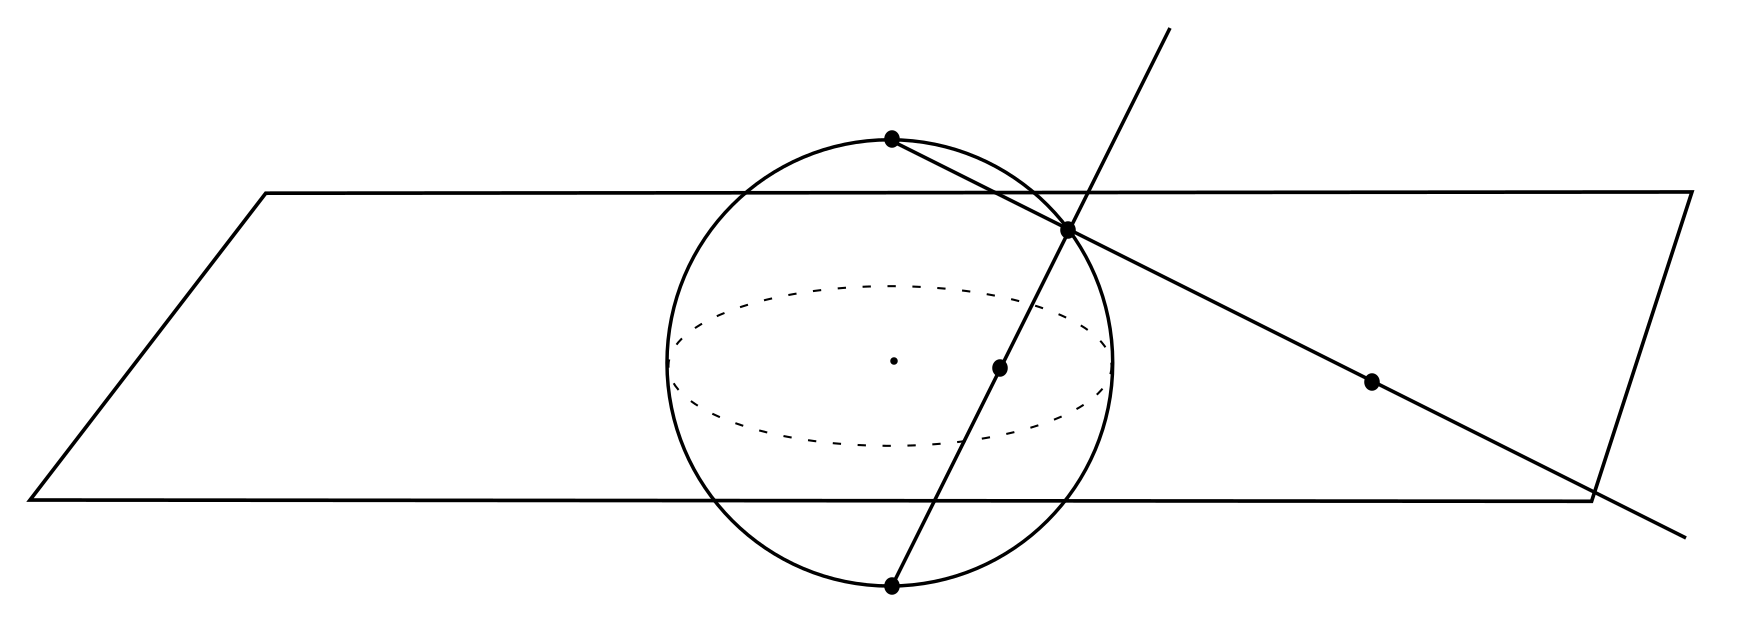
\includegraphics[width=150mm]{images/Exercises/stereotransition.png}
    \end{center}

    In other words, the map is given by $(x,y)\mapsto (\frac{x}{x^2+y^2},\frac{y}{x^2+y^2})$. If we do the computations, we find that the Jacobian is 

    $$J=\frac{1}{(x^2+y^2)^4}\det  \begin{pmatrix} y^2-x^2 & -2yx \\ -2yx & x^2-y^2  \end{pmatrix}=-\frac{1}{(x^2+y^2)^2}<0$$

    so this approach doesn't work...\newline

    \textbf{Attempt 2:} $S^2$ can be viewed as the level set of a smooth function $f: (x,y,z)\mapsto x^2+y^2+z^2$ with non-zero gradient and is therefore an orientable manifold.\newline

    \textbf{Attempt 3:} For those of you that would (for good reasons) argue that attempt 2 is somehow cheating because is doesn't use our definition, but rather a theorem we haven't presented, we will now present a proof using first principles. This will use a similar idea as in exercise (a). If we describe the sphere as the set of points $\{(\sin\phi \sin \theta ,\sin \phi \cos \theta, \cos \phi)\in \R^3 \} $. Let  $(U_1,\varphi_1)$ be the chart where...

    \item Show that the total space of the tangent bundle of a smooth n-manifold is an orientable
manifold. 
\end{enumerate}



\hspace{1cm}

\begin{exercise} \textbf{\textit{Computation of $\Omega_0^{\textrm{or}}$}}\\
Compute the oriented bordism group $\Omega_0^{\textrm{or}}$.
\end{exercise}

\noindent We have that $0$-dimensional oriented manifolds are classified by a finite collection of points, each with sign. By connecting points of different signs with oriented lines we get a cobordism to a finite collection of points all of the same sign. The sum of the signs in this sense is quite obviously invariant under cobordisms, and so we realise that $\Omega_0^{or}\cong \Z$.

\hspace{1cm}

\begin{exercise} \textbf{\textit{Computation of $\Omega_2^{\textrm{or}}$}}
	\begin{enumerate}[label=(\alph*)]
		\item Work through the argument in detail showing that \(\Sigma_g\) is cobordant to the empty
        set.
		\item Recall that the disjoint union is cobordant to the connected sum. Work through
        the details for an example different from what was shown in the lecture.
		\item Conclude that \(\Omega_2^{\textrm{or}} = 0\). (Here, you may omit details about the orientations of the
        3-dimensional cobordisms.)
	\end{enumerate}
\end{exercise}

\noindent Let us now try to understand this cobordism group in dimension 2 a bit better.

	\begin{enumerate}[label=(\alph*)]
		\item To understand that $\Sigma_g$ is cobordant to the empty set we will use the "standard" embedding in $\R^3$. The manifold with boundary that is the interior of this surface in $\R^3$ forms a cobordism between $\Sigma_g$ and $\emptyset$.
		\item Push along the normal bundle...
		\item This follows from classification of surfaces...
	\end{enumerate}

\newpage

\begin{exercise} \textbf{\textit{Computation of \(\Omega_2^{\textrm{unor}}\):}}
	\begin{enumerate}[label=(\alph*)]
		\item Show that the Klein bottle \(K\) is cobordant to the empty set. %See argument around Fig 4, Lec 1, Dan Freed
		\item (Poincaré duality and Euler characteristic) Show that \(\mathbb{R}\mathbb{P}^2\) is non-zero in \(\Omega_2^{\textrm{unor}}\), i.e. that there is no compact 3-manifold $X$ with boundary $\partial X = \R \mathbb{P}^2$. \\
        \textit{Hint:} Consider the double $D= X \underset{\R \mathbb{P}^2}{\cup} X$. What does Poincaré duality imply
        about the Euler characteristic of 3-dimensional closed manifolds?
		\item Conclude from the above that \(\Omega_2^{\textrm{unor}} = \mathbb{Z}/{2\mathbb{Z}}\).
	\end{enumerate}
\end{exercise}




\subsection*{Sheet 2.}

\begin{exercise} \textbf{\textit{Framings}}\\
Justify your answers to the following questions:
	\begin{enumerate}[label=(\alph*)]
	\item Can a Klein bottle be framed?
	  \item Can $S^2$ be framed?
          \item An \textbf{isotopy between the framings} is a deformation given by a family of framings parameterized by the interval. 
        Are any of the framed cylinders below isotopic? 
        \item Which of the framings induce the same orientations? 
	\end{enumerate}

 \begin{center} 
		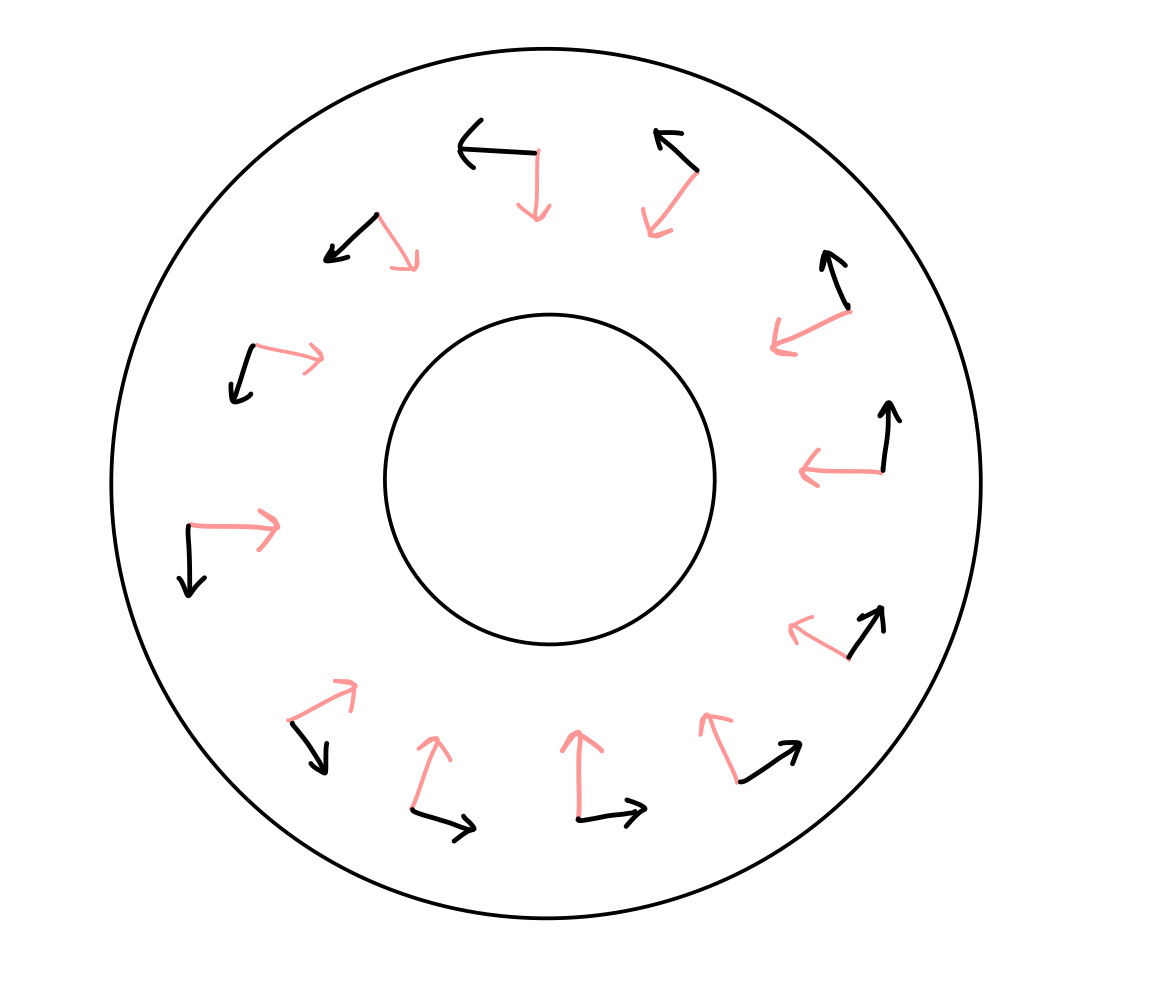
\includegraphics[scale=0.1]{images/Exercises/-1framing.jpeg}
            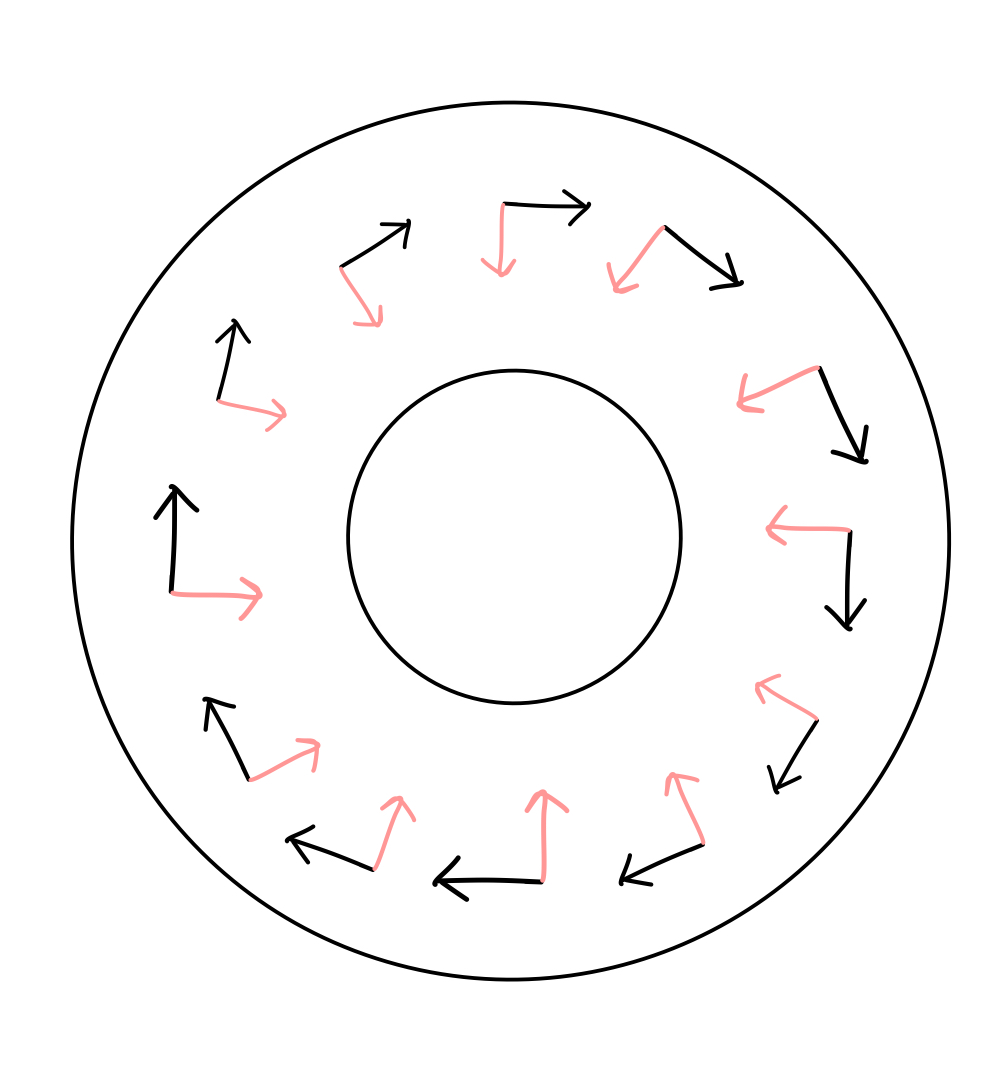
\includegraphics[scale=0.1]{images/Exercises/+1framing.jpeg}
            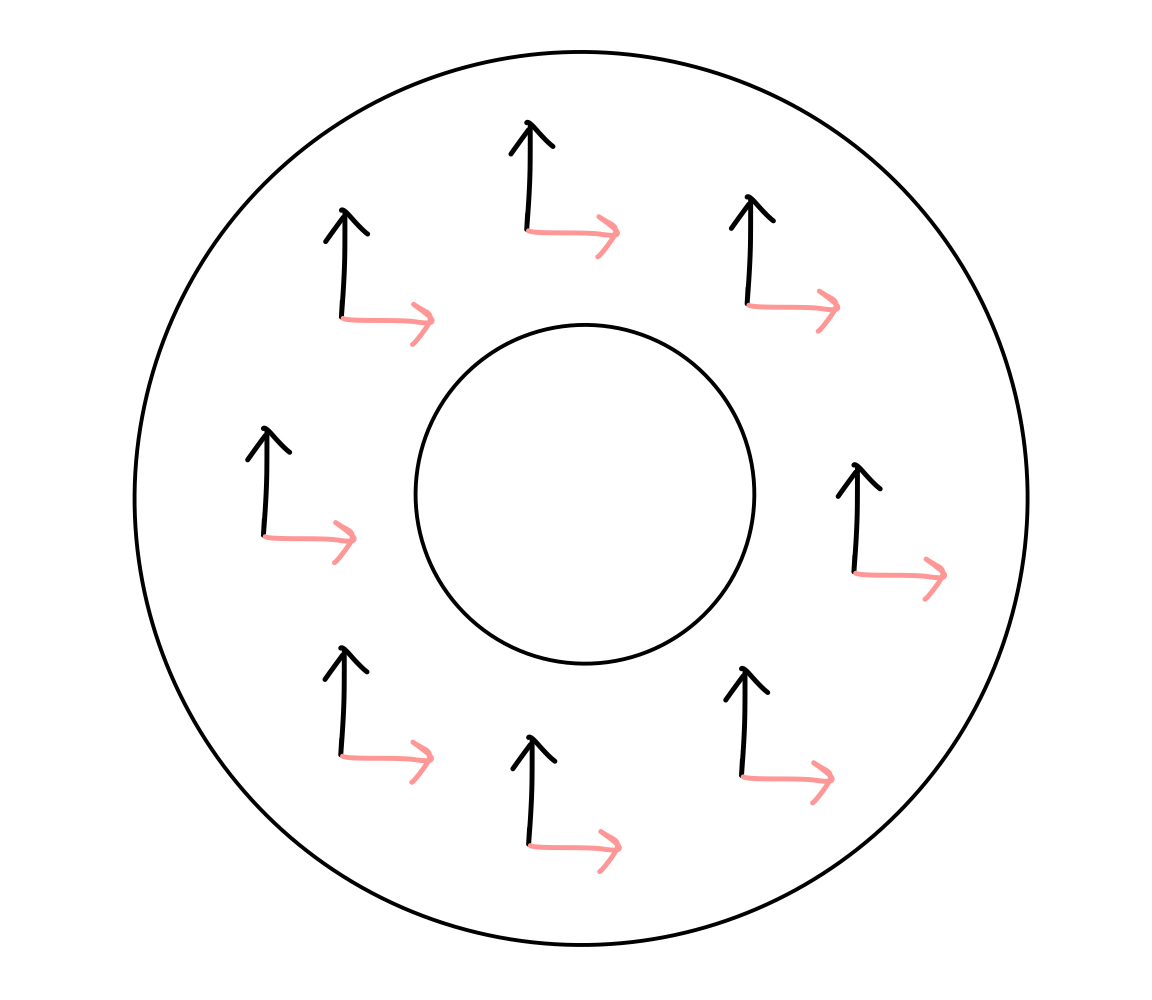
\includegraphics[scale=0.1]{images/Exercises/0framing.jpeg}

		\end{center}

  
\end{exercise}


\begin{enumerate}[label=(\alph*)]
	\item A Klein bottle cannot be framed because it is unoriented (existence of a framing is more restrictive).
	  \item $S^2$ can also not be framed even though it is orientable. This is a consequence of the hairy ball theorem.
          \item An \textbf{isotopy between the framings} is a deformation given by a family of framings parameterized by the interval. 
        Are any of the framed cylinders below isotopic? ...
        \item The two rightmost framings induce the same orientations.
	\end{enumerate}


\begin{exercise} \textbf{\textit{Attaching handles}}\\
\textbf{Definition.} Let \(B^n\) denote the \(n\)-dimensional ball as a manifold with boundary and \(S^n\) the \(n\)-dimensional sphere. 

Given a 2-dimensional manifold $M$, we {\em attach a \(j\)-handle} \(H^j\coloneq B^j \times B^{2-j}\), for \(j\in \{0,1,2\}\) via  and a smooth embedding \(f: S^{j-1}\times D^{2-j} \hookrightarrow \partial M\) as follows: 
\begin{align*}
	M\cup_f H^j \coloneq \big( M\sqcup (B^j \times B^{2-j}) \big) / \sim
\end{align*}
where for \((p,x) \in S^{j-1}\times B^{2-j} \subset B^j \times B^{2-j}\), we set \(f(p,x)\sim (p,x)\) . 
	\begin{enumerate}[label=(\alph*)]
	\item Convince yourself that there is a smooth structure on $M\cup_f H^j$.
	\item Which surface is obtained from attaching a 1-handle to a disk?
	\item Which surface is obtained from attaching two 1-handles to a disk, i.e.~from attaching an additional 1-handle to the surface obtained in part (a)?
	\item Build the torus by successively attaching handles to a disk.
	\end{enumerate}
\end{exercise}

	\begin{enumerate}[label=(\alph*)]
	\item "I can explain it to you, but I can't understand it for you."
	\item A cylinder (or a Moebius strip).
	\item A so-called pair of pants.
	\item To a disk we successively add a 1-handle, another 1-handle, and finally cap everything off with a 2-handle.
	\end{enumerate}




\begin{exercise} \textbf{\textit{Properties of the connected sum of manifolds}}
	\begin{enumerate}[label=(\alph*)]
        \item Given  \(n\)-manifolds \(M\), \(M'\), and \(M''\),  show that the connected sum satisfies the following properties.
	   \begin{enumerate}[label=(\roman*)]
		\item  \(M\# S^n \cong M\), \qquad\qquad\qquad\qquad\qquad {\em (neutral element)}
		\item  \(M\# M' \cong M'\# M\), and \qquad\qquad\qquad {\em (commutativity)}
		\item  \((M\# M') \# M'' \cong M\# (M' \# M'')\). \qquad {\em (associativity)}
	\end{enumerate}
	\item If \(M\) and \(M'\) are smooth \(n\)-manifolds, construct a smooth structure on the connected sum \(M\#M'\). Note that this is not unique but defines a well-defined diffeomorphism class.
	You may like to read more details using isotopies in Chapter 8, Section 2 in Hirsch, Differential Topology\footnote{Can e.g.~be accessed at \url{https://www.researchgate.net/publication/268035774_Differential_Topology}.}.
	\end{enumerate}
\end{exercise}


\hspace{1cm}

\begin{exercise} \textbf{\textit{Reading exercise}}\\
Below is a list of several proofs of the classification theorem of 1-dimensional manifolds using different tools. Read through one (or several) of them, or find your own. 
	\begin{enumerate}[label=(\roman*)]
		\item \url{https://pnp.mathematik.uni-stuttgart.de/igt/eiserm/lehre/2014/Topologie/Gale\%20-\%201-manifolds.pdf}
		\item Appendix of  \url{https://www.maths.ed.ac.uk/~v1ranick/papers/milnortop.pdf}, starting at p.55. 
	\end{enumerate}
\end{exercise}




\subsection*{Sheet 3.}

\begin{exercise} \textbf{\textit{Morse functions}}
	\begin{enumerate}[label=(\alph*)] 
	\item Consider the function \(f: \mathbb{R}^2 \rightarrow \mathbb{R}\) given by \((x,y)\mapsto x^3-3xy^2\). Find all the critical points and check if $f$ is a Morse function. If it does not meet the criteria, perturb it in such a way that it becomes a Morse function.
	\item Consider the function \(f:\mathbb{R}^2 \rightarrow \mathbb{R}\) defined by \((x,y)\mapsto x^2y^2\). Find all the critical points and check if $f$ is a Morse function. If it does not meet the criteria, perturb it in such a way that it becomes a Morse function.
	\item Show that if \(f:M \rightarrow \mathbb{R}\) and \(g: N\rightarrow \mathbb{R}\) are Morse functions, then \(f+g: M\times N \rightarrow \mathbb{R}\) is also a Morse function, and the critical points are pairs of critical points of \(f\) and \(g\). Visualize this for $M=N=S^1$ and $f\colon S^1 \subset \R^2\to \R$ the projection onto the first coordinate. 
\end{enumerate}
\end{exercise}

\begin{enumerate}[label=(\alph*)] 
	\item We have that $\grad f=(3x^2-3y^2,-6xy)$, and so the only critical point is the origin. The Hessian determinant is $$\mathscr{H}=\det \begin{pmatrix}
	    6x & -6y \\ -6y & -6x
	\end{pmatrix}$$ and hence degenerate at the origin. This means $f$ is not Morse. We can perturb it by adding $\varepsilon (x^2+y^2)$ for a sufficiently small $\varepsilon>0$ such that it becomes Morse. This has the origin as its only critical point and adds $2 \varepsilon I_2$ to the Hessian matrix, thus making the determinant not vanish at the origin.

 
	\item By, again, computing the gradient $\grad f=(2xy^2,2yx^2)$, we realise that the set of critical points of $f$ consists precisely of the $x$- and $y$-axis. Therefore, $f$ is obviously not Morse. 
	\item Show that if \(f:M \rightarrow \mathbb{R}\) and \(g: N\rightarrow \mathbb{R}\) are Morse functions, then \(f+g: M\times N \rightarrow \mathbb{R}\) is also a Morse function, and the critical points are pairs of critical points of \(f\) and \(g\). Visualize this for $M=N=S^1$ and $f\colon S^1 \subset \R^2\to \R$ the projection onto the first coordinate. 
\end{enumerate}




\begin{exercise} \textbf{\textit{Handle decomposition}}\\
\textbf{Definition 1.} Let \(M\) be a compact 2-manifold. A \textbf{handle decomposition} of \(M\) is a finite sequence of manifolds 
\begin{align*}
\emptyset = W_{-1} \subseteq W_0 \subseteq W_1 \subseteq W_2 = M
\end{align*}
 such that each \(W_i\) is obtained from \(W_{i-1}\) by attaching \(i\)-handles. 
\begin{enumerate}[label=(\alph*)] 
            \item Find two different handle decompositions of \(S^2\). 	
		\item Find a handle decomposition of \(\mathbb{R}\mathbb{P}^2\). 
		\item Find a handle decomposition of the Klein bottle. 
		\item  Explain why, for any non-empty closed connected surface, we can start a handle decomposition with a single 0-handle. \textit{Hint}: The key argument was mentioned in lectures as ``\emph{handle cancellation}".
		\item Using the idea of handle cancellation, bring the surface below into {\em normal form}, i.e.~such that read from bottom to top, the index of the critical points are non-decreasing.
		\begin{center}
			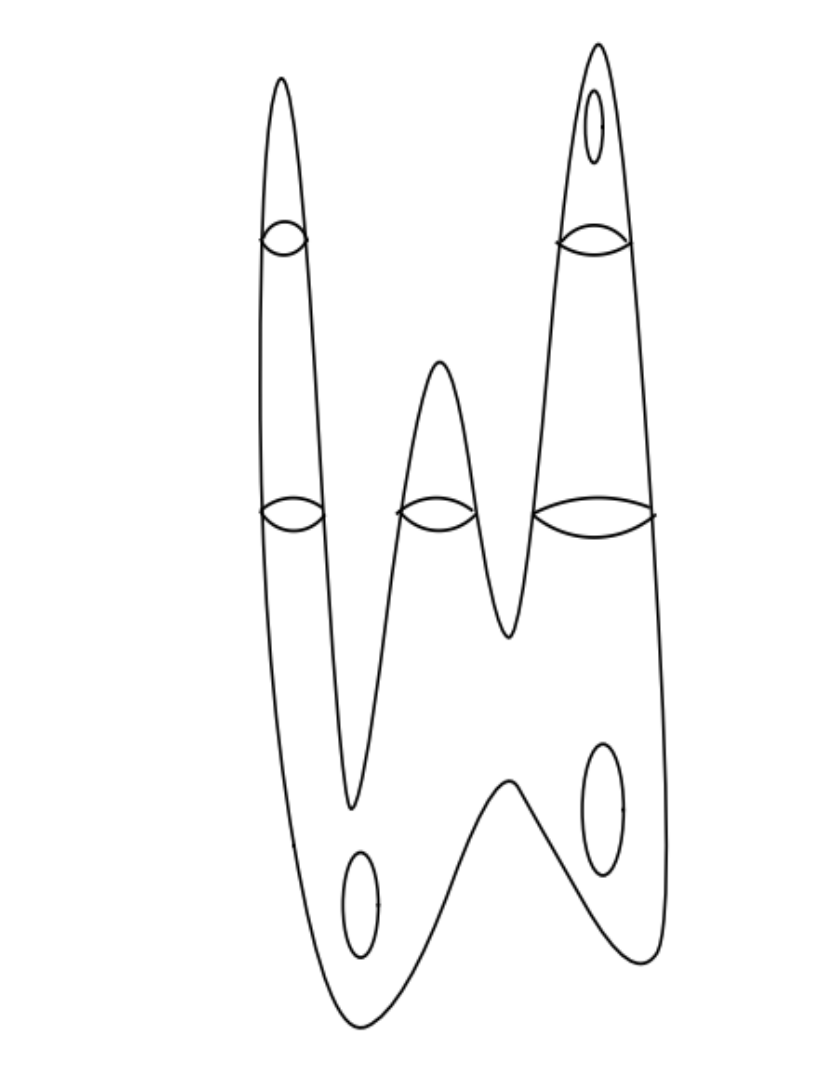
\includegraphics[scale=0.3]{images/Exercises/FunkyTorus.png}
		\end{center}
\end{enumerate}

\end{exercise}

\hspace{1cm}

\begin{exercise} \textbf{\textit{Reading exercise - Classification of closed 1-manifolds}}\\
Prove the following theorem using Morse theory and/or read through the proof in \url{https://www.math.csi.cuny.edu/~abhijit/papers/classification.pdf} [Theorem 15]. 
	\begin{thm}
			Any closed 1-manifold is homeomorphic to \(S^1\).
        \end{thm}

\end{exercise}







